%%%%%%%%%%%%%%%%%%%%%%%%%%%%%%%%%%%%%%%%%
% Beamer Presentation
% LaTeX Template
% Version 1.0 (10/11/12)
%
% This template has been downloaded from:
% http://www.LaTeXTemplates.com
%
% License:
% CC BY-NC-SA 3.0 (http://creativecommons.org/licenses/by-nc-sa/3.0/)
%
%%%%%%%%%%%%%%%%%%%%%%%%%%%%%%%%%%%%%%%%%

%----------------------------------------------------------------------------------------
%	PACKAGES AND THEMES
%----------------------------------------------------------------------------------------

%\documentclass[mathserif]{beamer}
\documentclass[handout]{beamer}

\mode<presentation> {

% The Beamer class comes with a number of default slide themes
% which change the colors and layouts of slides. Below this is a list
% of all the themes, uncomment each in turn to see what they look like.

%\usetheme{default}
%\usetheme{AnnArbor}
\usetheme{Antibes} %++
%\usetheme{Bergen}
%\usetheme{Berkeley}
%\usetheme{Berlin}
%\usetheme{Boadilla}
%\usetheme{CambridgeUS} %+
%\usetheme{Copenhagen}
%\usetheme{Darmstadt} %++
%\usetheme{Dresden}
%\usetheme{Frankfurt}
%\usetheme{Goettingen}
%\usetheme{Hannover}
%\usetheme{Ilmenau} %++
%\usetheme{JuanLesPins}
%\usetheme{Luebeck}
%\usetheme{Madrid}
%\usetheme{Malmoe}
%\usetheme{Marburg}
%\usetheme{Montpellier}
%\usetheme{PaloAlto}
%\usetheme{Pittsburgh}
%\usetheme{Rochester}
%\usetheme{Singapore}
%\usetheme{Szeged}
%\usetheme{Warsaw}

% As well as themes, the Beamer class has a number of color themes
% for any slide theme. Uncomment each of these in turn to see how it
% changes the colors of your current slide theme.

%\usecolortheme{albatross}
\usecolortheme{beaver}
%\usecolortheme{beetle}
%\usecolortheme{crane}
%\usecolortheme{dolphin}
%\usecolortheme{dove}
%\usecolortheme{fly}
%\usecolortheme{lily}
%\usecolortheme{orchid}
%\usecolortheme{rose}
%\usecolortheme{seagull}
%\usecolortheme{seahorse}
%\usecolortheme{whale}
%\usecolortheme{wolverine}

%\setbeamertemplate{footline} % To remove the footer line in all slides uncomment this line
\setbeamertemplate{footline}[frame number] % To replace the footer line in all slides with a simple slide count uncomment this line

\setbeamertemplate{navigation symbols}{} % To remove the navigation symbols from the bottom of all slides uncomment this line
}

\usepackage{graphicx} % Allows including images
\usepackage{booktabs} % Allows the use of \toprule, \midrule and \bottomrule in tables
\usepackage[utf8x]{inputenc}
\usepackage[spanish]{babel}
\usepackage{tikz,times}
\usepackage{multicol}
\usepackage{verbatim}
\usetikzlibrary{mindmap,trees,backgrounds}

  % Keys to support piece-wise uncovering of elements in TikZ pictures:
  % \node[visible on=<2->](foo){Foo}
  % \node[visible on=<{2,4}>](bar){Bar}   % put braces around comma expressions
  %
  % Internally works by setting opacity=0 when invisible, which has the 
  % adavantage (compared to \node<2->(foo){Foo} that the node is always there, hence
  % always consumes space plus that coordinate (foo) is always available.
  %
  % The actual command that implements the invisibility can be overriden
  % by altering the style invisible. For instance \tikzsset{invisible/.style={opacity=0.2}}
  % would dim the "invisible" parts. Alternatively, the color might be set to white, if the
  % output driver does not support transparencies (e.g., PS) 
  %
\tikzset{
    invisible/.style={opacity=0},
    visible on/.style={alt={#1{}{invisible}}},
    alt/.code args={<#1>#2#3}{%
      \alt<#1>{\pgfkeysalso{#2}}{\pgfkeysalso{#3}} % \pgfkeysalso doesn't change the path
    },
  }

%----------------------------------------------------------------------------------------
%	TITLE PAGE
%----------------------------------------------------------------------------------------

\title[Evaluación de modelos de aprendizaje automático
para posicionamiento indoor utilizando Bluetooth
low energy]{Evaluación de modelos de aprendizaje automático
para posicionamiento indoor utilizando Bluetooth
low energy\\\normalsize Trabajo de Memoria} % The short title appears at the bottom of every slide, the full title is only on the title page

\author{Felipe Berrios Toloza} % Your name
\institute[UTFSM] % Your institution as it will appear on the bottom of every slide, may be shorthand to save space
{
Universidad Técnica Federico Santa María \\ % Your institution for the title page
\medskip
\textit{felipe.berriost@alumnos.usm.cl} % Your email address
}
\date{11 de abril de 2018} % Date, can be changed to a custom date

\begin{document}

\begin{frame}
\titlepage % Print the title page as the first slide
\end{frame}

\begin{frame}{Tabla de Contenidos}
\begin{multicols}{2}
  \tableofcontents
\end{multicols}
\end{frame}


\AtBeginSection[]
{
  \begin{frame}{Tabla de Contenidos}
   \begin{multicols}{2}
     \tableofcontents[currentsection,hideothersubsections]
   \end{multicols}
  \end{frame}
}

%----------------------------------------------------------------------------------------
%	PRESENTATION SLIDES
%----------------------------------------------------------------------------------------

%------------------------------------------------
\section{Introducción} 
%------------------------------------------------

\begin{frame}
\frametitle{Introducción}

\textbf{Geolocalización}
\begin{itemize}

%\item La geolocalización ha jugado un papel fundamental en las últimas décadas.

\item Desde la edad antigua, múltiples formas de localización han sido desarrolladas.

\item Dentro de los avances más importantes en este ámbito, es el desarrollo de la teoría científica y técnica denominada georreferenciación.

\item Gracias a GPS, el crecimiento y acceso de la georreferenciación y navegación está en progresivo aumento.

\item Motivación: Georreferenciar dentro de una explotación minera, donde no hay alcance de señales GPS.

\end{itemize}



\end{frame}


%------------------------------------------------
\subsection{Definición del problema}

\begin{frame}
\frametitle{Definición del problema}

\begin{itemize}

\item Es necesario posicionamiento en interiores.

\pause
\item Cuando se usa tecnología GPS dentro de edificios o bajo tierra, existen muchos obstáculos e interferencia que imposibilitan su uso.

\pause
\item Sistemas de posicionamiento actuales (IPS) presentan problemas ya que confían en indicadores de fuerza de la señal (RSSI) para estimar distancias.

\end{itemize}

\pause
\vspace*{.5cm}
\textbf{Problema: Mejorar exactitud de sistemas de posicionamiento en interiores mediante modelos que aprendan de las señales}

\end{frame}

%------------------------------------------------

\subsection{Objetivos} % A subsection can be created just before a set of slides with a common theme to further break down your presentation into chunks

\begin{frame}
\frametitle{Objetivos}

\begin{itemize}
%\item Evaluar calidad de las señales \textit{Bluetooth Low Energy}, tanto en precisión como exactitud.

\item Diseñar un método de mapeo para un área mediante señales RSSI (\textit{fingerprint}).
\pause
\item Comparar métodos de aprendizaje automático sobre mediciones RSSI para determinar cuál posee menor error y es más exacto en posicionamiento indoor.
\pause
\item Determinar que tanto afectan los métodos de reducción de dimensionalidad al problema.

\end{itemize}

\end{frame}

%------------------------------------------------
\section{Estado del Arte}
%------------------------------------------------

\subsection{Tecnologías para posicionamiento \textit{indoor}}
\begin{frame}
\frametitle{Tecnologías para posicionamiento \textit{indoor}}

 % The "c" option specifies centered vertical alignment while the "t" option is used for top vertical alignment
 
\begin{itemize}
\item Basado en Visión
\item Infrarrojo
\item Tecnologías basadas en Sonido
\item RFID
\end{itemize}

\end{frame}

%-------------------------------------------------------------
\begin{frame}

\frametitle{Tecnologías Inalámbricas}

WiFi, Bluetooth, ZigBee, UWB, FM, GSM

\begin{block}{Received Signal Strength Indicator}
RSSI es una escala de referencia para medir el nivel de potencia de la fuerza de la señal recibida por el receptor. Se mide en dBm donde 0 RSSI indica señal ideal y valores más negativos indican mayor perdida. 
\end{block}

\begin{block}{Tx Power}
Es la potencia de salida o fuerza de la señal que el emisor produce durante el tiempo de transmisión. A mayor Tx Power, más estable es la señal, pero más energía se consume.
\end{block}
\end{frame}

%------------------------------------------------
\subsection{Técnicas  matemáticas Wireless para localización indoor}
\begin{frame}
\frametitle{Proximidad}

\begin{itemize}

\item Es el método más simple, y se basa en determinar una posición simbólica y aproximada de la posición del usuario.

\item Antenas o emisores de ondas de radio. Según la señal más fuerte detectada por el usuario, es donde se localiza en el sistema.

\item Ampliamente usado en redes celulares. GSM, Infrarrojo, Cell-ID.
\end{itemize}


\end{frame}

%------------------------------------------------

\begin{frame}
\frametitle{Triangulación}

\begin{figure}
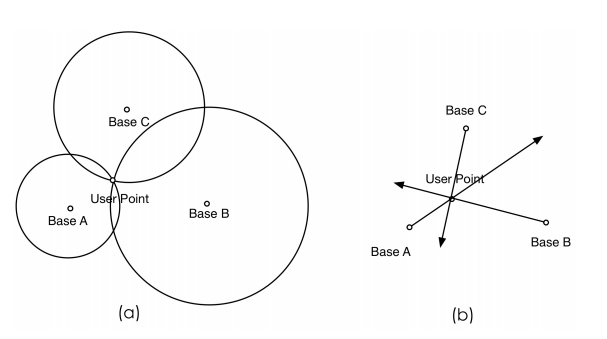
\includegraphics[width=\linewidth]{../figures/triangulacion.png}
\end{figure}

\end{frame}

%------------------------------------------------

\begin{frame}
\frametitle{Fingerprint}

\begin{figure}
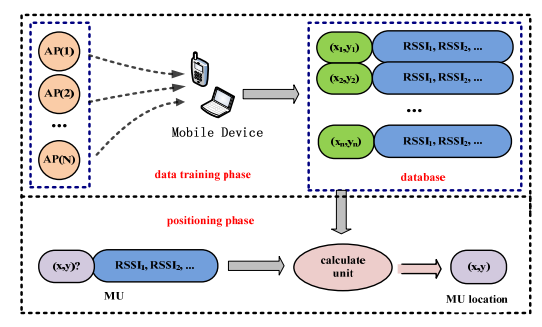
\includegraphics[width=.8\linewidth]{../figures/finger.png}
\end{figure}

\end{frame}


%------------------------------------------------
\section{Propuesta de solución}
%------------------------------------------------

\begin{frame}
\frametitle{Propuesta}

\begin{itemize}
\item Establecer un marco de trabajo para la recolección, entrenamiento y clasificación de algoritmos de machine learning utilizando Bluetooth Low Energy.\\

\pause

\item Comparación de diferentes clasificadores.\\

\pause
\item Utilizar técnicas de reducción de dimensionalidad.\\
\pause

\item Utilizar modelos sin necesidad de conexión a internet.
\end{itemize}

\end{frame}


%------------------------------------------------
\subsection{Consideraciones Previas}

\begin{frame}
\frametitle{Beacons}

\begin{columns}[t] % The "c" option specifies centered vertical alignment while the "t" option is used for top vertical alignment

\column{.5\textwidth} % Left column and width

\begin{itemize}
\item La transmisión corresponde a un ID único que está presente en cada Beacon y que no se repite, como una dirección MAC o un UUID.

\item Auge del Internet de las cosas.

\item Habitualmente los Beacons soportan ambos protocolos existentes, es decir IBeacon y Eddystone.

\end{itemize}

\column{.5\textwidth} % Right column and width
\begin{figure}
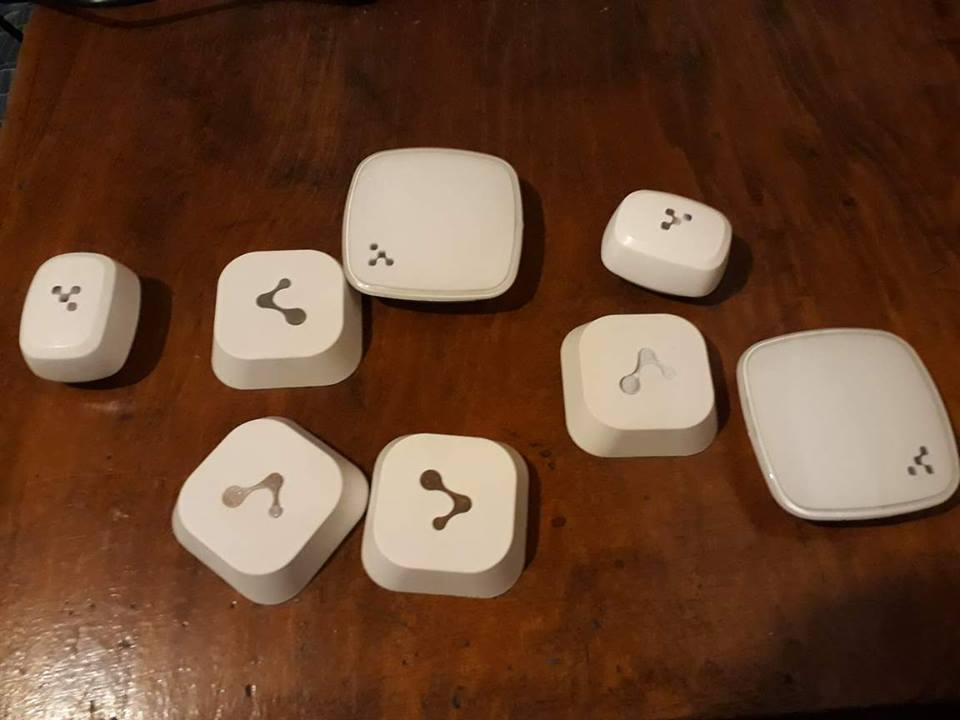
\includegraphics[width=\textwidth]{../figures/beacons_all.jpg}

\end{figure}

\end{columns}

\end{frame}

%------------------------------------------------
\subsection{Descripción del \textit{framework} de posicionamiento}
\begin{frame}
\frametitle{Descripción del \textit{framework} de posicionamiento}

\begin{itemize}

\item Establecer un marco de trabajo.

\pause

\item Se utiliza la técnica de Fingerprint discutida en el estado del arte, mediante la utilización de un mapa de señales, también denominado \textit{radiomap}.

\pause

\item Utilizar dispositivos Bluetooth Low Energy. Luego, el procedimiento se divide en las dos clásicas etapas de Fingerprint, es decir, fase \textit{offline} y fase \textit{online}.
\end{itemize}


\end{frame}

%------------------------------------------------

\begin{frame}
\frametitle{Fase Offline}

\begin{figure}
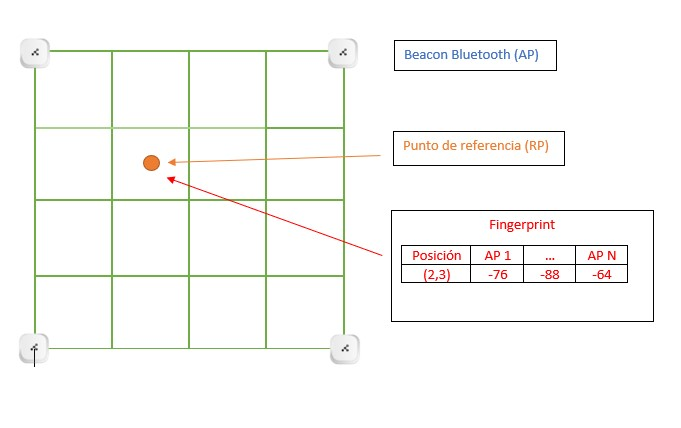
\includegraphics[width=\textwidth]{../figures/fingerprints.jpg}
\end{figure}

\end{frame}

%-------------------------------------------------

\begin{frame}
\frametitle{Entrenamiento de algoritmos}

\begin{itemize}

\item Entrenar técnicas de máquinas de aprendizaje.

\pause
\item Posteriormente, se seleccionan los mejores algoritmos y luego son implementados.
\pause

\item Reducción de dimensionalidad
\pause

\item \textbf{¿Implementación en cliente o servidor?}

\end{itemize}

\end{frame}

%-------------------------------------------------

\begin{frame}
\frametitle{Fase Online}

\begin{itemize}

\item Para la fase online se reconocen dos etapas principales.

\begin{enumerate}
\pause
\item Colectar un vector de señales RSSI en la posición actual del usuario.
\pause
\item Proveer este vector de entrada a los algoritmos de aprendizaje supervisado ya entrenados.
\end{enumerate}

\pause
\item La misma aplicación de la fase offline, es utilizada para mostrar en un mapa de tiempo real la localización actual de usuario.

\end{itemize}
\end{frame}


%-------------------------------------------------

\begin{frame}
\frametitle{Proceso de desarrollo}

\begin{figure}
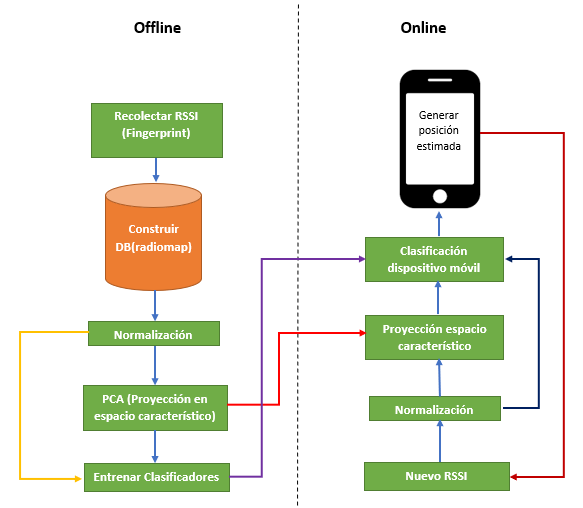
\includegraphics[width=0.7\textwidth]{../figures/propuesta_memoria.png}
\end{figure}


\end{frame}

%-------------------------------------------------
\section{Experimentación}
%-------------------------------------------------

\subsection{Implementación}

\begin{frame}
\frametitle{Beacons y configuración}

\begin{columns}[t] % The "c" option specifies centered vertical alignment while the "t" option is used for top vertical alignment

\column{.5\textwidth} % Left column and width
\begin{figure}
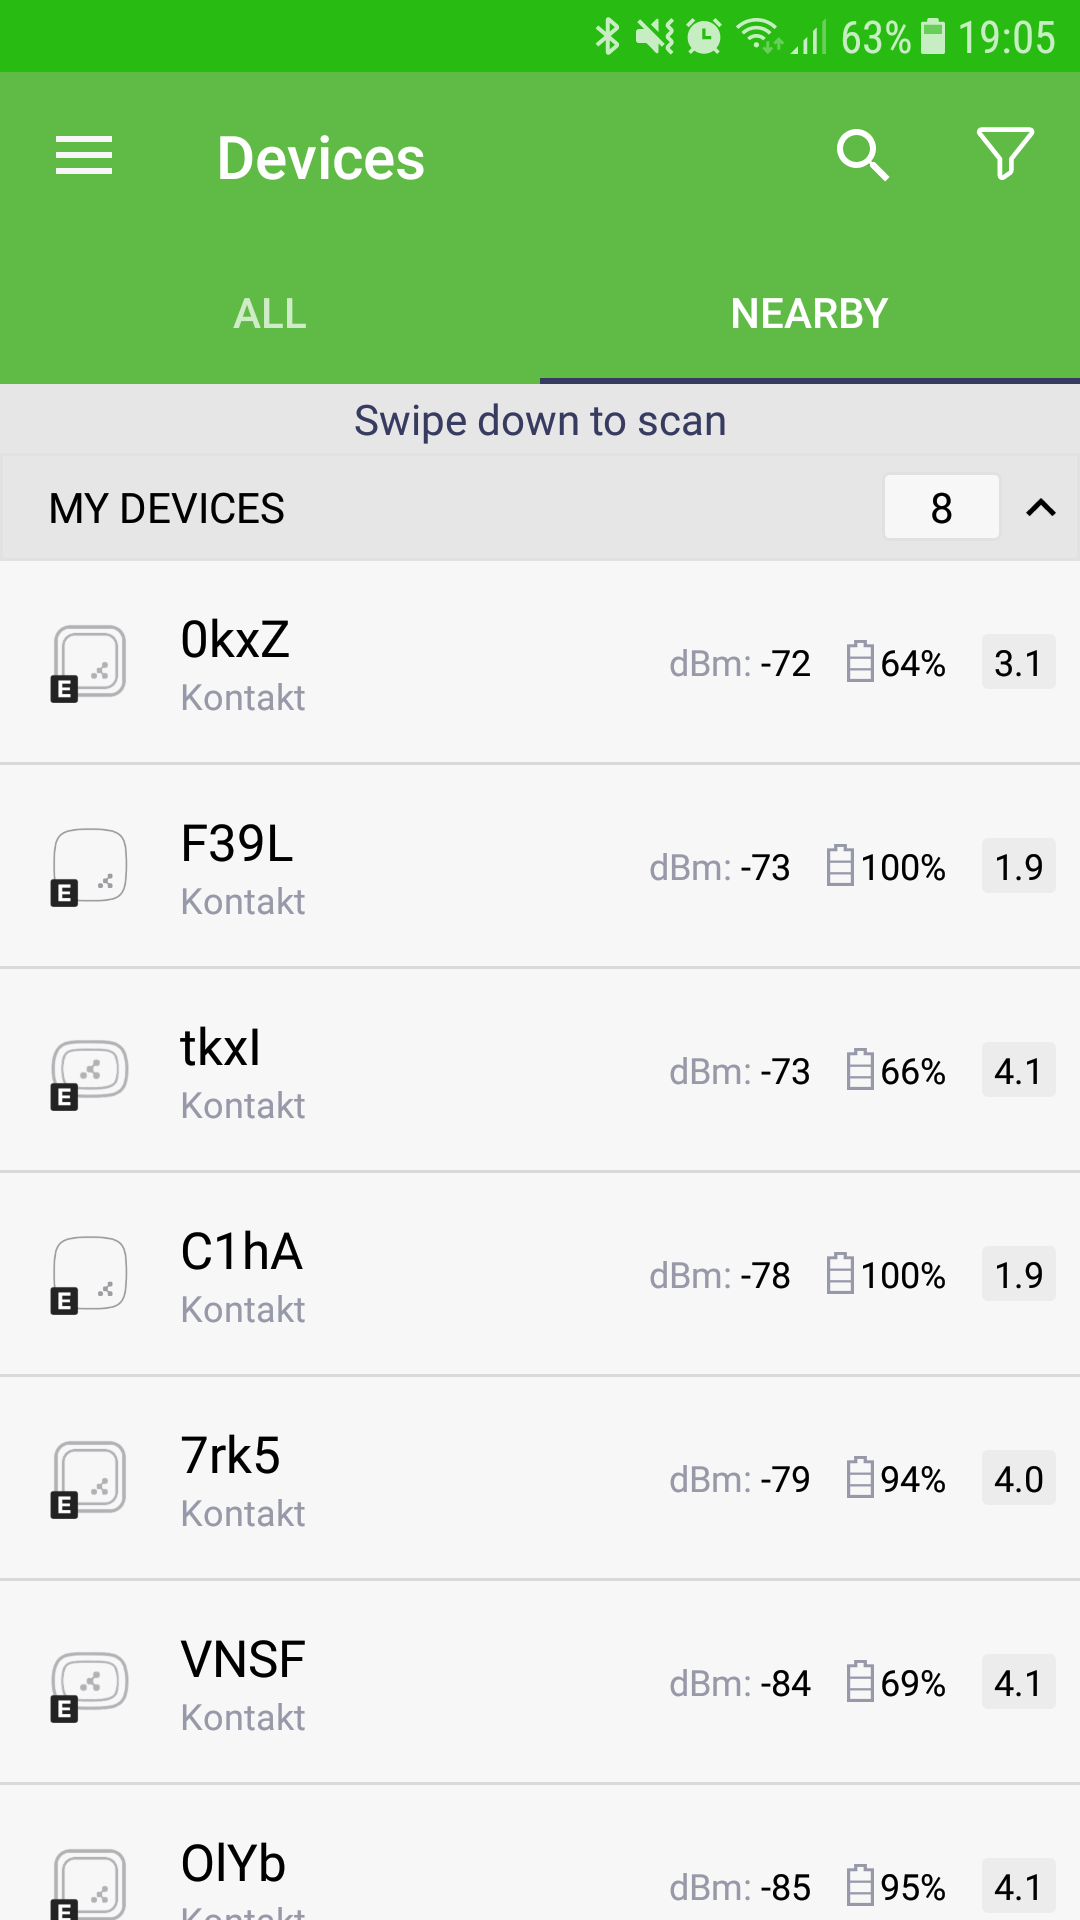
\includegraphics[width=0.6\textwidth]{../figures/kontaktapp1.png}
\end{figure}

\column{.5\textwidth} % Right column and width
\begin{figure}
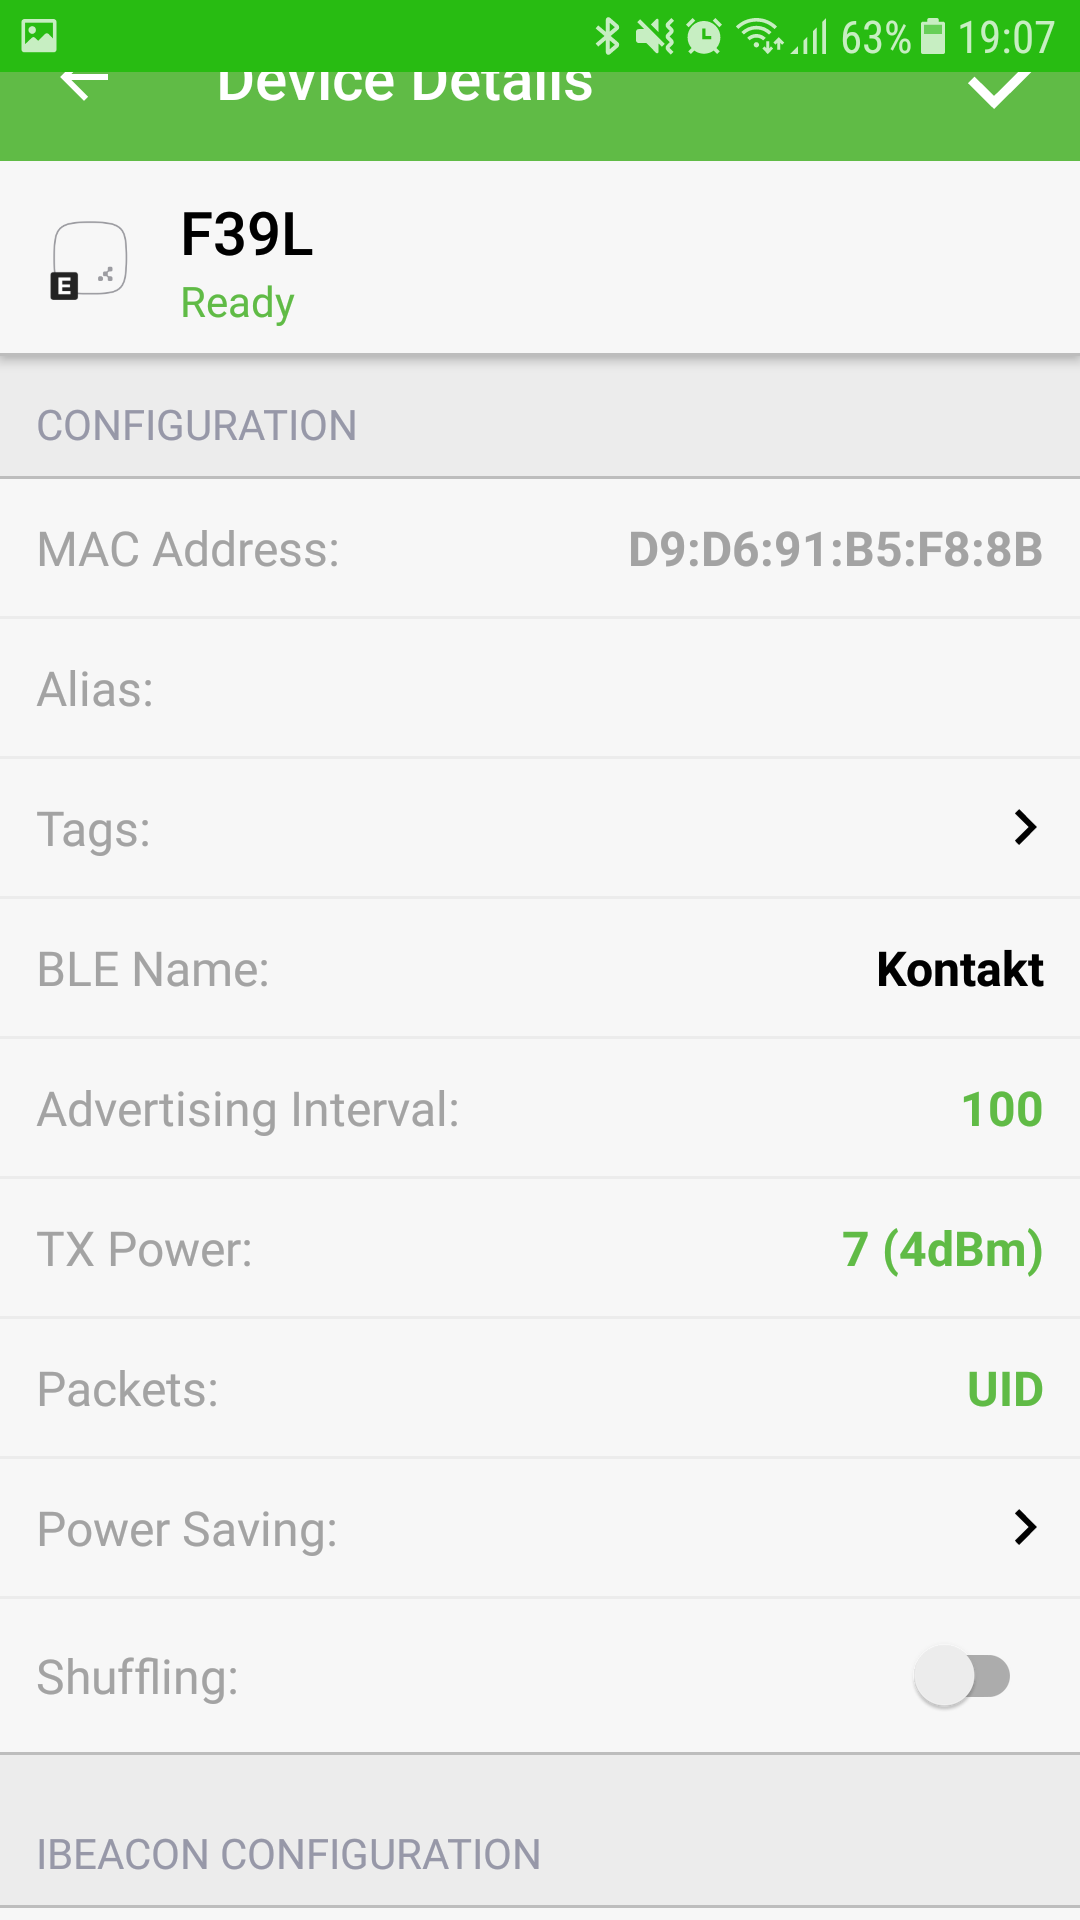
\includegraphics[width=0.6\textwidth]{../figures/kontaktapp2.png}
\end{figure}

\end{columns}
\end{frame}
%------------------------------------------------

\begin{frame}
\frametitle{Lugar de experimentación}

Estacionamiento subterráneo de la universidad Técnica Federico Santa María, Campus San Joaquín.

\begin{columns}[t] % The "c" option specifies centered vertical alignment while the "t" option is used for top vertical alignment

\column{.5\textwidth} % Left column and width
\begin{figure}
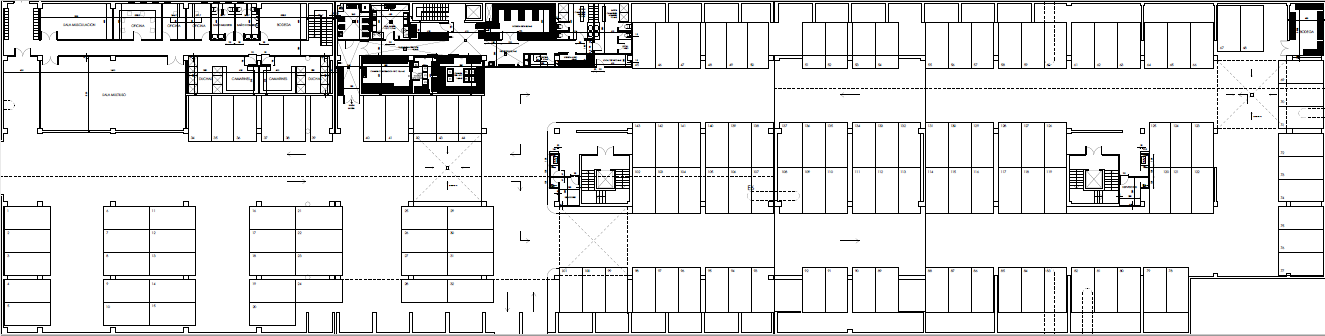
\includegraphics[width=\textwidth]{../figures/estSubterraneo.png}
\end{figure}

\column{.5\textwidth} % Right column and width
\begin{figure}
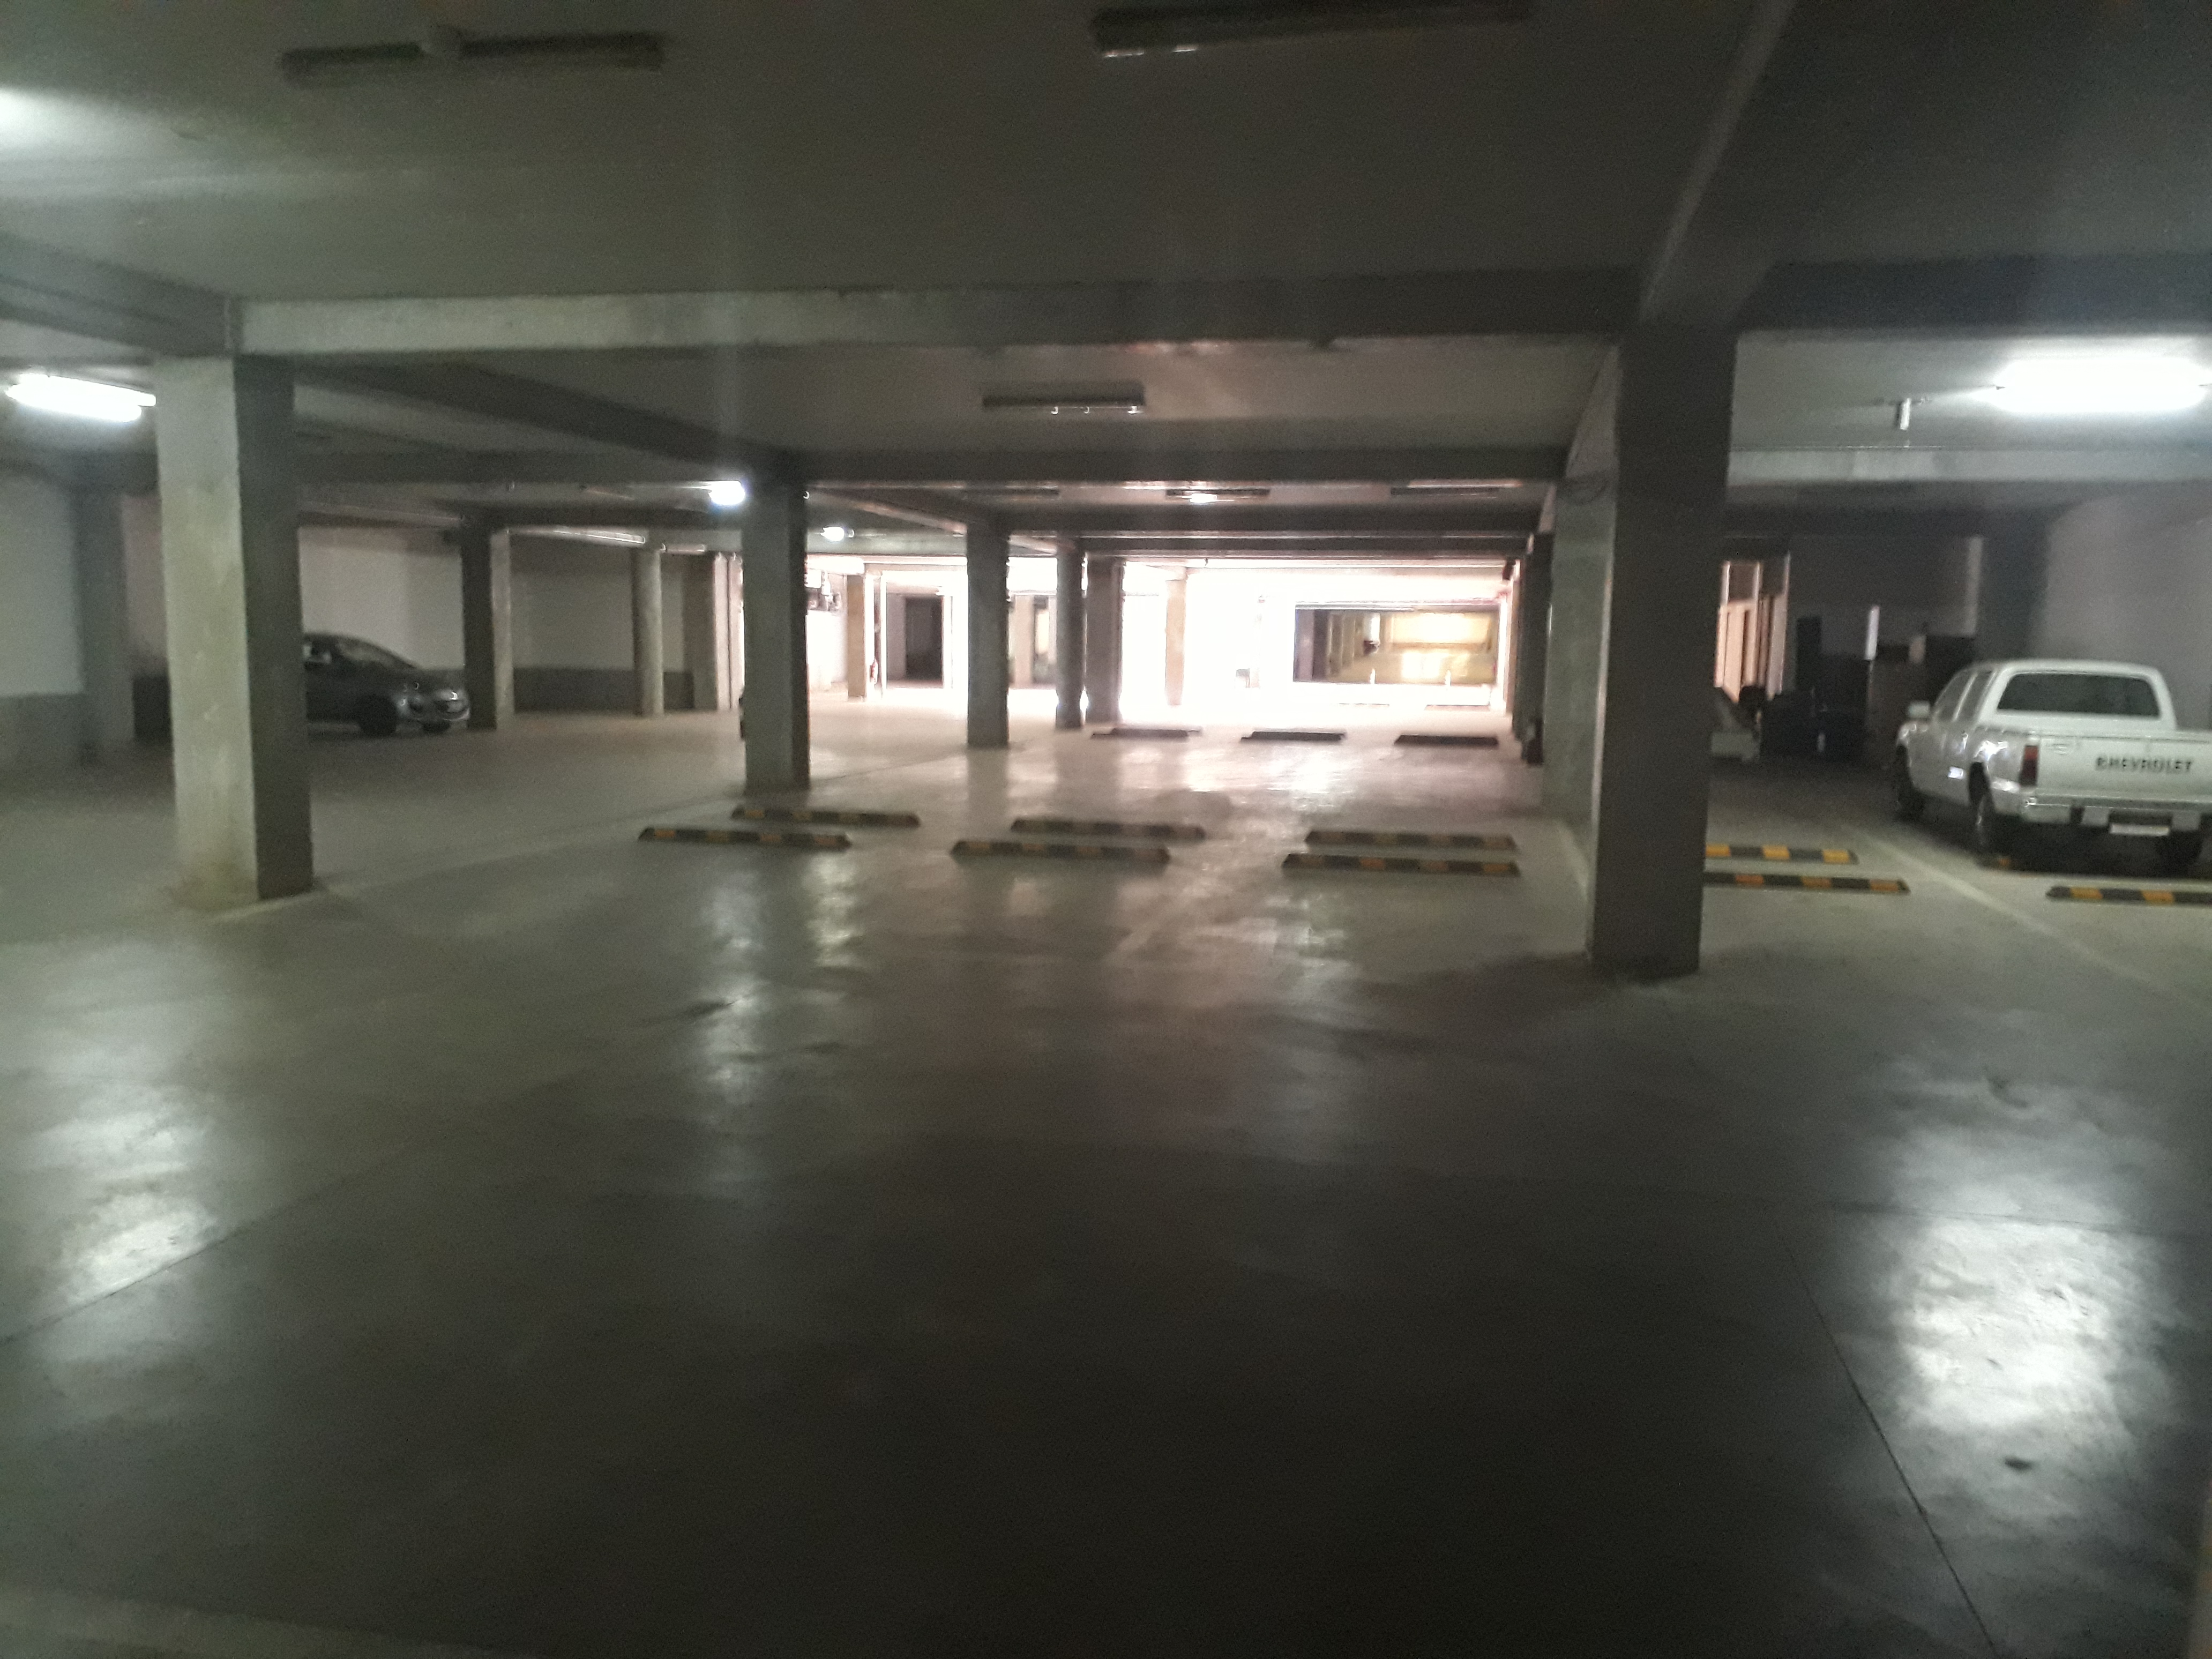
\includegraphics[width=\textwidth]{../figures/estReal.jpg}
\end{figure}

\end{columns}

\end{frame}

%------------------------------------------------

\begin{frame}
\frametitle{Software Utilizado}

\begin{itemize}
\item Aplicación Android
	
\pause

\item Scikit-learn

\pause

\item Tensorflow

\end{itemize}

\end{frame}

%------------------------------------------------

\begin{frame}
\frametitle{Recolección de Fingerprints}

\begin{columns}[t] % The "c" option specifies centered vertical alignment while the "t" option is used for top vertical alignment

\column{.7\textwidth} % Left column and width

\begin{itemize}
\item Samsung Galaxy J7 Prime,CPU Octa-core 1.6 GHz, 3GB de memoria ram interna y el tipo de Bluetooth corresponde a 4.1 LE

\item 8 beacons en un área reducida del estacionamiento. 16 x 44 metros ($704m^2$).

\item Grilla para los puntos de referencia de 4 metros por 4 metros, 44 en total.

\item Se obtiene una base de datos \textit{SQLite} con Figerprints, la cual presenta 6600 registros.
\end{itemize}

\column{.5\textwidth} % Right column and width
\begin{figure}
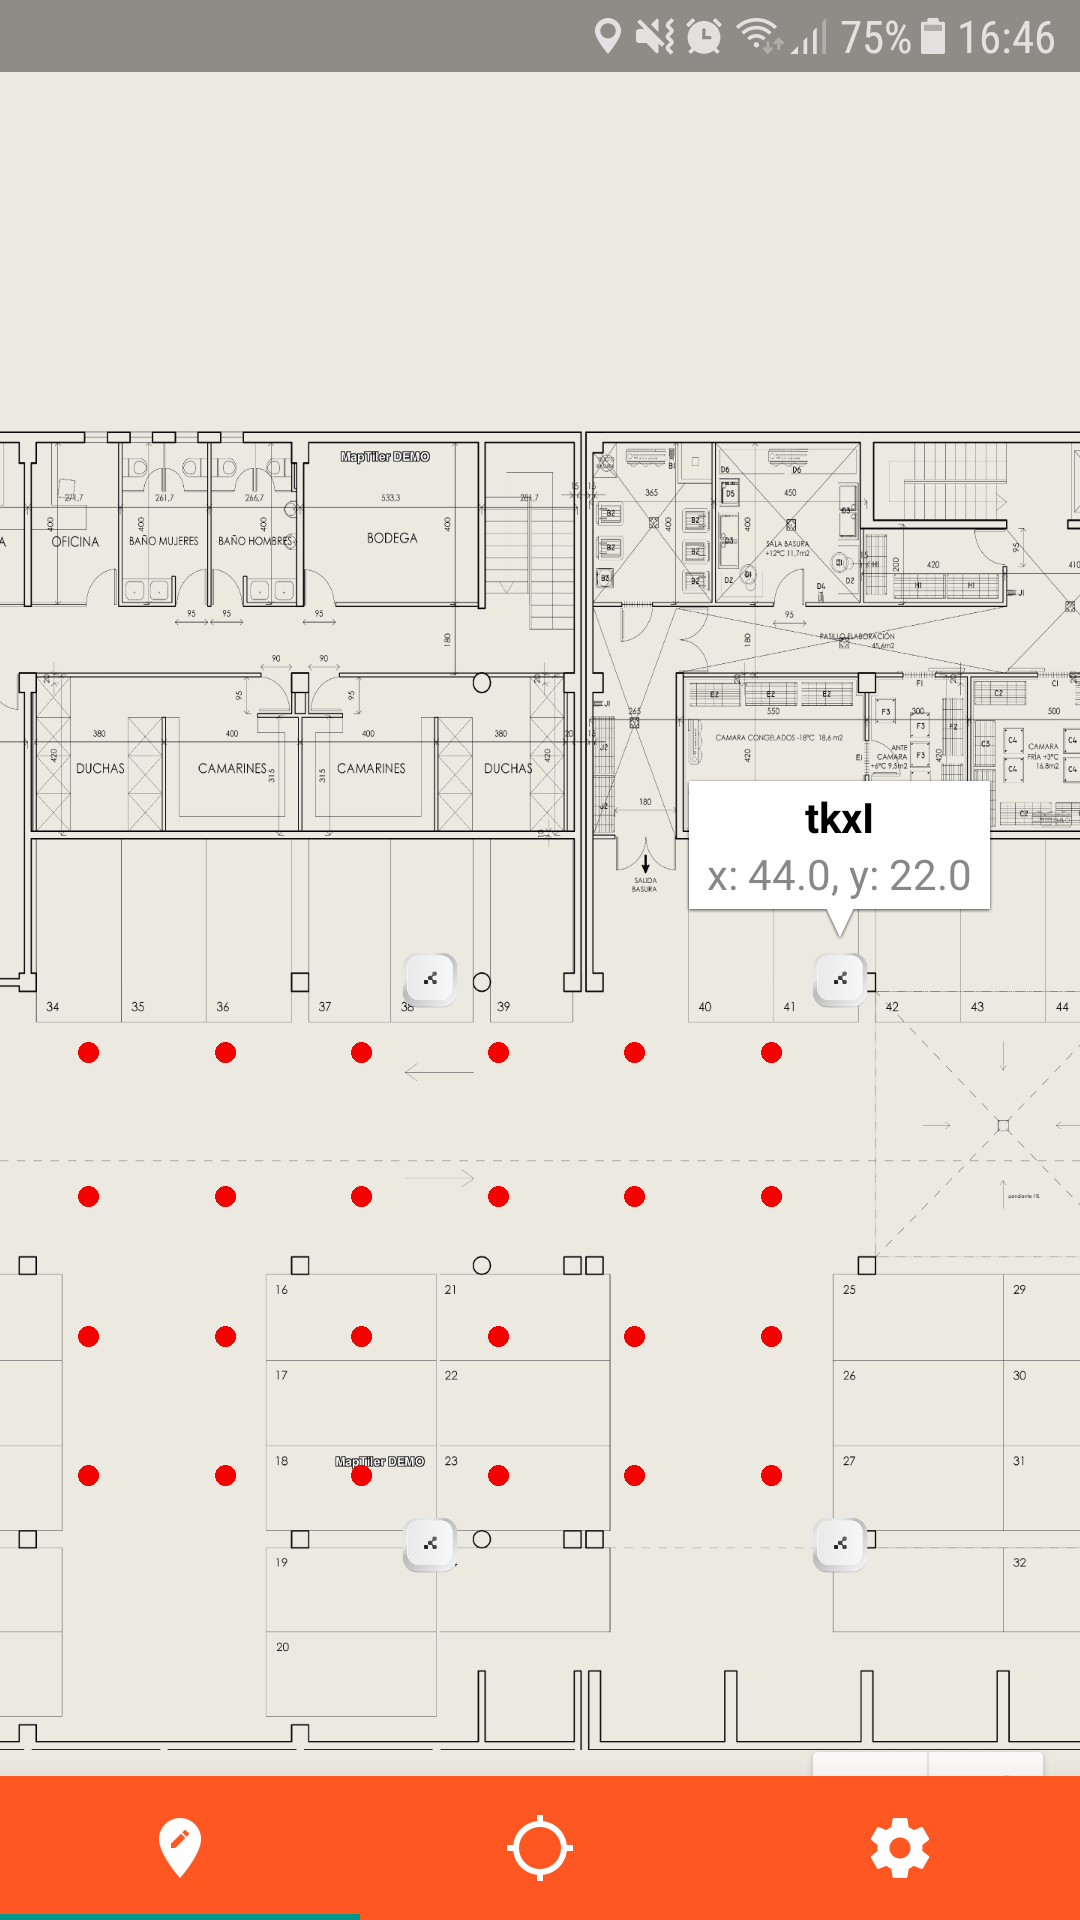
\includegraphics[width=0.65\textwidth]{../figures/deployBeacons.png}
\end{figure}

\end{columns}

\end{frame}

%-------------------------------------------------
\begin{frame}
\frametitle{Entrenamiento de clasificadores}

\begin{columns}[t] 
\column{.5\textwidth} % Left column and width

\begin{figure}
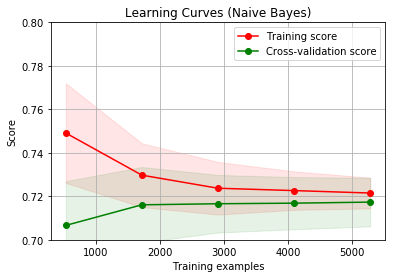
\includegraphics[width=\textwidth]{../figures/NB.png}
\end{figure}

\column{.5\textwidth} % Right column and width
\begin{figure}
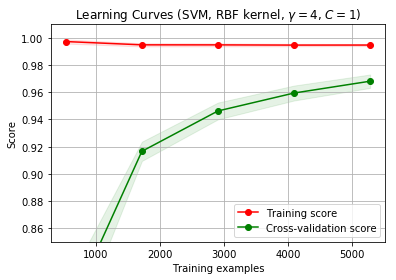
\includegraphics[width=\textwidth]{../figures/SVM-RBF.png}
\end{figure}

\end{columns}


\end{frame}

%-------------------------------------------------
\begin{frame}
\frametitle{Entrenamiento de clasificadores}

\begin{itemize}
\item Red utilizada es una red neuronal profunda con dos capas ocultas, la primera de ellas tiene 256 neuronas o nodos, mientras que la segunda capa posee 64 neuronas.

\item 20000 epoch, \textit{learning rate}  igual a $\alpha = 0.3$ . También se define un \textit{batch size} igual a 32.
\end{itemize}
\begin{columns}[t] 
\column{.5\textwidth} % Left column and width

\begin{figure}
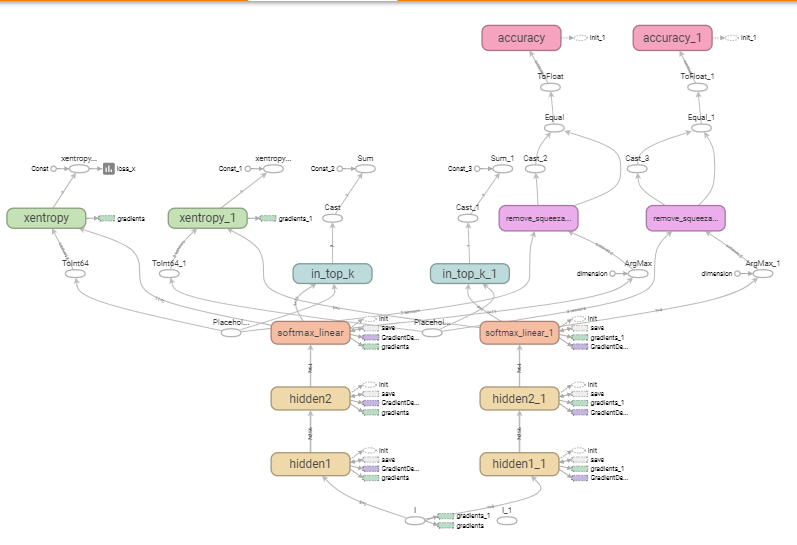
\includegraphics[width=\textwidth]{../figures/nn_estructura.png}
\end{figure}



\column{.5\textwidth} % Right column and width
\begin{figure}
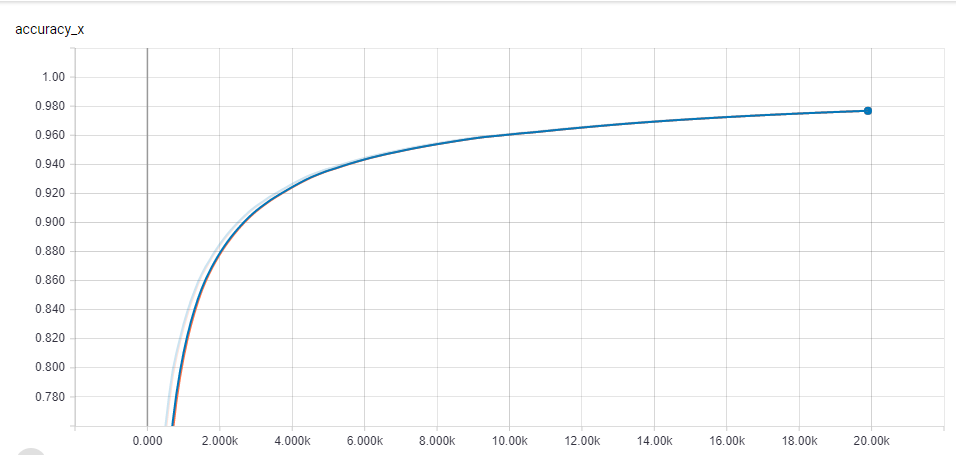
\includegraphics[width=\textwidth]{../figures/nn_plot.png}
\end{figure}

\end{columns}


\end{frame}


%-------------------------------------------------
\begin{frame}
\frametitle{Tabla de entrenamiento}

\begin{table}[ht!]
\centering
\resizebox{\textwidth}{!}{%
\begin{tabular}{|c|c|c|c|c|}
\hline
Algoritmo                     & Accuracy & Error medio X & Error medio Y & Error Absoluto \\ \hline
NN                            & 97.94\%  & 0.1579        & 0.0735        & 0.1741         \\ \hline
$SVM(RBF, C=1, \gamma = 4)$   & 96.81\%  & 0.2254        & 0.1018        & 0.2473         \\ \hline
$KNN(k = 2)$                  & 95.43\%  & 0.9842        & 0.1575        & 0.9967         \\ \hline
QDA                           & 85.25\%  & 5.1103        & 4.7175        & 6.9548         \\ \hline
$SVM(Lineal, C=1)$            & 78.75\%  & 9.3163        & 6.0387        & 11.1022        \\ \hline
Random Forest                 & 77.33\%  & 11.3430       & 3.1409        & 11.7698        \\ \hline
Naive Bayes                   & 71.73\%  & 12.2303       & 9.4836        & 15.4763        \\ \hline
Decision Tree( max depth = 5) & 57.91\%  & 57.8012       & 5.6412        & 58.0758        \\ \hline
Adaboost                      & 26.03\%  & 150.8848      & 6.5333        & 151.0261       \\ \hline
\end{tabular}
}
\end{table}


\end{frame}

%-------------------------------------------------
\begin{frame}
\frametitle{Entrenamiento utilizando PCA}

Determinar número de componentes principales que deben ser utilizadas.

\begin{columns}[t] % The "c" option specifies centered vertical alignment while the "t" option is used for top vertical alignment

\column{.5\textwidth} % Left column and width

\begin{figure}
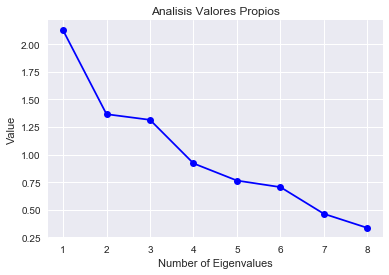
\includegraphics[width=\textwidth]{../figures/eigenvalues.png}
\end{figure}

\column{.5\textwidth} % Right column and width
\begin{figure}
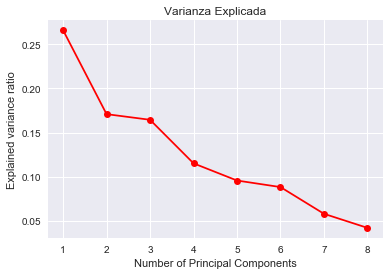
\includegraphics[width=\textwidth]{../figures/varianza_ratio.png}
\end{figure}
 % Right column and widt

\end{columns}

\end{frame}

%-------------------------------------------------
\begin{frame}
\frametitle{Entrenamiento utilizando PCA}

Tres criterios: Valores propios, Varianza explicada y Clasificadores

\begin{figure}
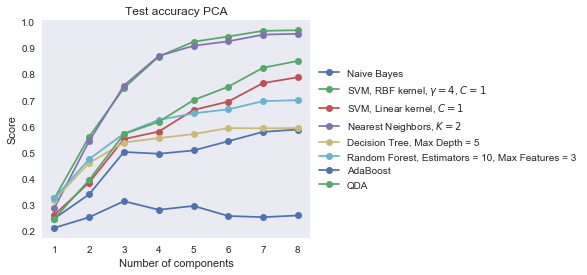
\includegraphics[width=\textwidth]{../figures/comparativa_clasificadores_pca.png}
\end{figure}


\end{frame}

%-------------------------------------------------
\begin{frame}
\frametitle{Entrenamiento utilizando PCA}

\begin{table}[ht!]
\centering
\resizebox{\textwidth}{!}{%
\begin{tabular}{|c|c|c|c|c|}
\hline
Algoritmo                     & Accuracy & Error medio X & Error medio Y & Error Absoluto \\ \hline
NN                            & 93\%  & 1.8956        & 0.6589        & 2.0068         \\ \hline
$SVM(RBF, C=1, \gamma = 4)$   & 92.39\%  & 2.4581  & 0.7830        & 2.5797         \\ \hline
$KNN(k = 2)$                  & 90.83\%  & 2.1381 & 0.4872        & 2.1929         \\ \hline
QDA                           & 71.25\%  & 15.9418 & 9.3042        & 18.4583         \\ \hline
$SVM(Lineal, C=1)$            & 66.20\%  & 19.5878 & 10.4824        & 22.2162        \\ \hline
Random Forest                 & 64.15\%  & 21.3284 & 5.4472        & 22.0130       \\ \hline
Decision Tree( max depth = 5) & 56.96\%  & 33.5151       & 8.9163       & 34.6808        \\ \hline
Naive Bayes                   & 50.71\%  & 31.3406 & 10.0727        & 32.9194        \\ \hline
Adaboost                      & 32.20\%  & 73.9345 & 9.3042       & 74.5176       \\ \hline
\end{tabular}
}
\end{table}


\end{frame}


%-------------------------------------------------
\begin{frame}
\frametitle{Fase Online}

\begin{itemize}
\item No hay forma de determinar el error absoluto, producto de que para ello se debe proporcionar la posición real.

\pause
\item Lo que se propone para determinar los resultados son dos formas llamadas método estático y método dinámico.
\end{itemize}

\end{frame}

%-------------------------------------------------
\begin{frame}
\frametitle{Fase Online}

\begin{columns}[t] % The "c" option specifies centered vertical alignment while the "t" option is used for top vertical alignment

\column{.3\textwidth} % Left column and width
\begin{figure}
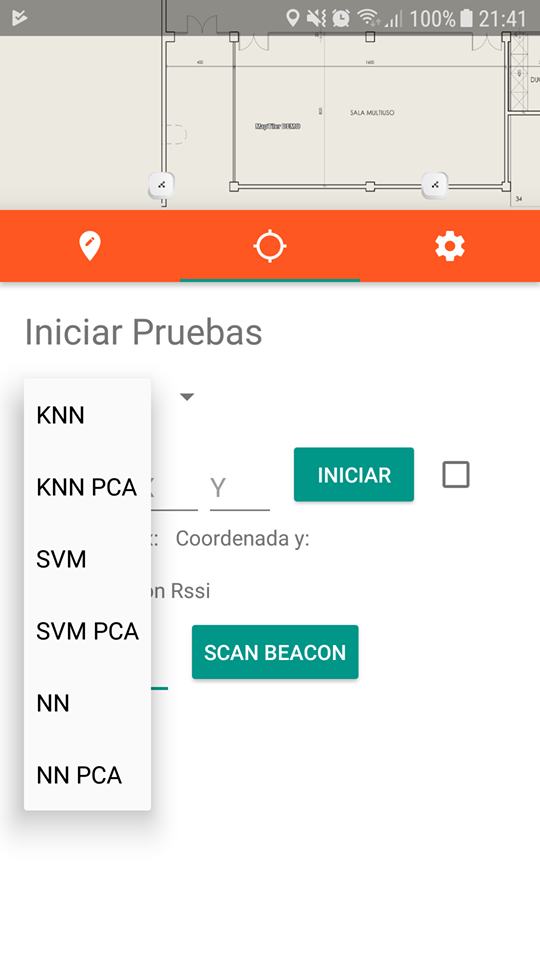
\includegraphics[width=\textwidth]{../figures/fase_online1.png}
\end{figure}

\column{.3\textwidth} % Right column and width
\begin{figure}
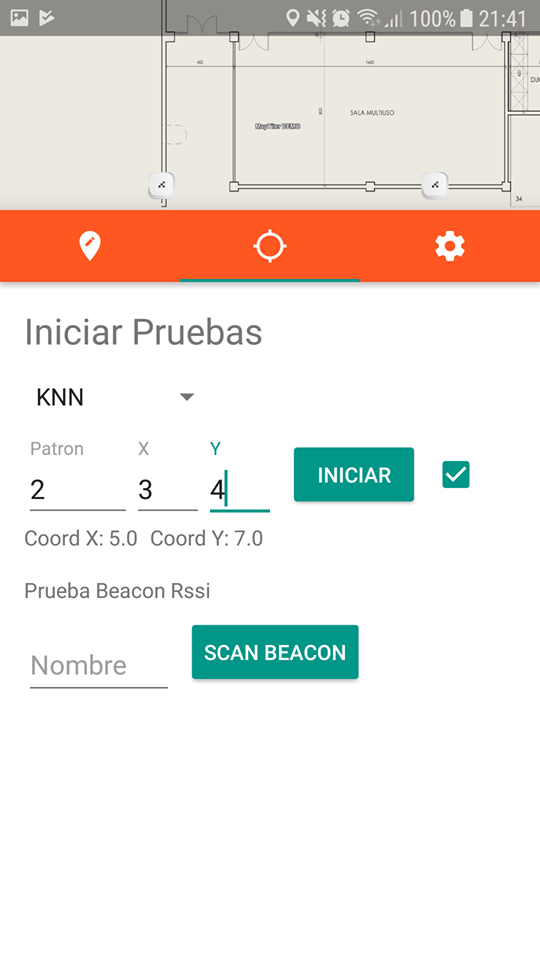
\includegraphics[width=\textwidth]{../figures/fase_online2.png}
\end{figure}

\column{.3\textwidth} % Right column and width
\begin{figure}
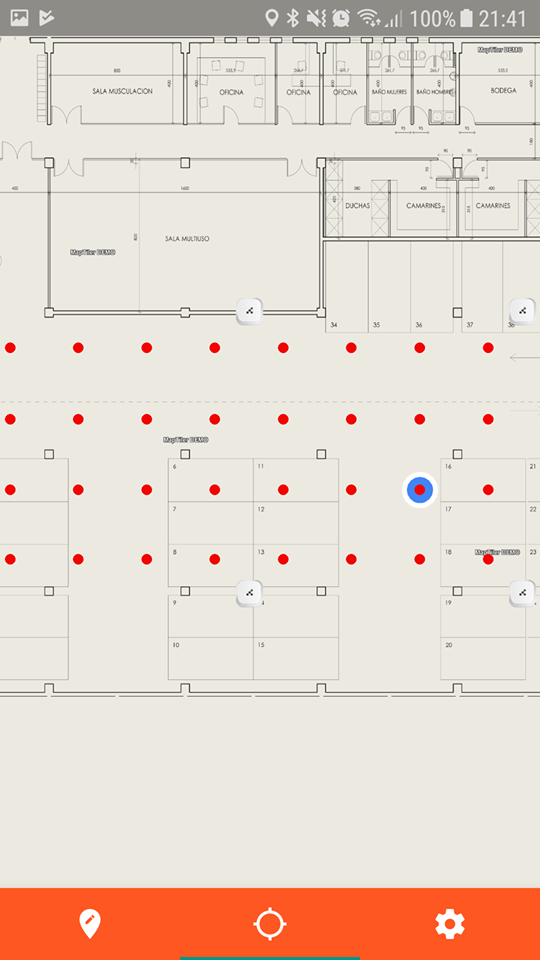
\includegraphics[width=\textwidth]{../figures/fase_online3.png}
\end{figure}

\end{columns}

\end{frame}

%-------------------------------------------------
\section{Resultados}
%-------------------------------------------------

\subsection{Métricas Obtenidas}
\begin{frame}
\frametitle{Errores medios método dinámico}

Método dinámico sin PCA

\begin{table}[ht!]
\centering
\resizebox{\textwidth}{!}{%
\begin{tabular}{|c|c|c|c|c|c|}
\hline
Clasificador & Error x & Error y & Varianza x & Varianza y & RMSE    \\ \hline
KNN          & 1.5858  & 4.6391  & 7.1970     & 2.1780     & 6.9323  \\ \hline
SVM          & 6.8207  & 2.8874  & 1.7243     & 0.5989     & 10.0323 \\ \hline
NN           & 4.3784  & 3.9113  & 13.0950    & 5.0712     & 8.2994  \\ \hline
\end{tabular}
}
\end{table}

Método dinámico con PCA
\begin{table}[!ht]
\centering
\resizebox{\textwidth}{!}{%
\begin{tabular}{|c|c|c|c|c|c|}
\hline
Clasificador & Error x & Error y & Varianza x & Varianza y & RMSE   \\ \hline
KNN PCA      & 2.0023  & 4.3983  & 7.5113     & 2.0696     & 6.6812 \\ \hline
SVM PCA      & 6.8948  & 2.4257  & 4.1134     & 2.0348     & 9.5668 \\ \hline
NN PCA       & 5.8874  & 4.4513  & 8.6088     & 3.2089     & 9.5188 \\ \hline
\end{tabular}
}
\end{table}


\end{frame}

%-------------------------------------------------
\begin{frame}
\frametitle{Errores medios método estático}

Método estático sin PCA

\begin{table}[!h]
\centering
\resizebox{\textwidth}{!}{%
\begin{tabular}{|c|c|c|c|c|c|}
\hline
Clasificador & Error x & Error y & Varianza x & Varianza y & RMSE   \\ \hline
KNN          & 3.2385  & 1.5417  & 3.3321     & 1.0940     & 5.0520 \\ \hline
SVM          & 5.2493  & 1.6986  & 2.0598     & 0.7594     & 7.0241 \\ \hline
NN           & 3.7300  & 2.1937  & 5.8885     & 0.7373     & 4.4857 \\ \hline
\end{tabular}
}
\end{table}

Método estático con PCA
\begin{table}[!h]
\centering
\resizebox{\textwidth}{!}{%
\begin{tabular}{|c|c|c|c|c|c|}
\hline
Clasificador & Error x & Error y & Varianza x & Varianza y & RMSE   \\ \hline
KNN PCA      & 2.9892  & 1.4475  & 3.1487     & 1.6391     & 5.0340 \\ \hline
SVM PCA      & 3.2313  & 1.4905  & 3.0630     & 1.7817     & 5.1757 \\ \hline
NN PCA       & 1.5578  & 1.7488  & 3.8045    & 2.6885     & 3.9341 \\ \hline
\end{tabular}
}
\end{table}

\end{frame}
%-------------------------------------------------
\begin{frame}
\frametitle{Cumulative distribution function Dinámico 100\%}

$$
F_{X} (x) = P(X \le x)
$$

\begin{table}[!h]
\centering
\resizebox{\textwidth}{!}{%
\begin{tabular}{|c|c|c|c|}
\hline
Clasificador & Sin PCA & Con PCA & Mejora     \\ \hline
KNN          & 16.576  & 16.1554 & 2.5374 \%  \\ \hline
SVM          & 20.8962 & 19.3874 & 7.2204 \%  \\ \hline
NN           & 20.5677 & 16.1554 & 21.4525 \% \\ \hline
\end{tabular}
}
\end{table}

\end{frame}

%-------------------------------------------------
\begin{frame}
\frametitle{Cumulative distribution function Estático 100\%}

$$
F_{X} (x) = P(X \le x)
$$

\begin{table}[!h]
\centering
\resizebox{\textwidth}{!}{%
\begin{tabular}{|c|c|c|c|}
\hline
Clasificador & Sin PCA  & Con PCA & Cambio    \\ \hline
KNN          & 16.1554  & 16.1554 & 0 \%      \\ \hline
SVM          & 16.1554  & 15.1327 & 6.33 \%   \\ \hline
NN           & 11.18033 & 16.1554 & -44.49 \% \\ \hline
\end{tabular}
}
\end{table}

\end{frame}

%-------------------------------------------------
\begin{frame}
\frametitle{Análisis de distribución}

\begin{figure}
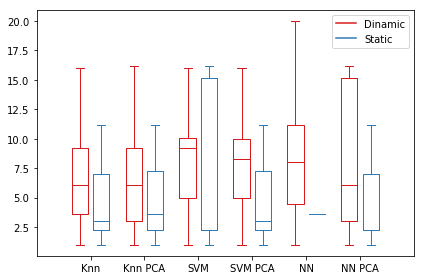
\includegraphics[width=\textwidth]{../figures/boxplot.png}
\end{figure}

\end{frame}

%-------------------------------------------------
\begin{frame}
\frametitle{Análisis tiempos de ejecución}

Resultados en términos de milisegundos con su respectiva mejora.

\begin{table}[ht!]
\centering
\resizebox{\textwidth}{!}{%
\begin{tabular}{|c|c|c|c|}
\hline
\textbf{Clasificador} & \textbf{Sin PCA} & \textbf{Con PCA} & \textbf{Incremento} \\ \hline
KNN                   & 64.9642          & 59.6786          & 8.1361\%            \\ \hline
SVM                   & 54.5985          & 25.6085          & 53.0966\%           \\ \hline
NN                    & 0.7610           & 0.5777           & 24.0867\%           \\ \hline
\end{tabular}
}
\end{table}

\end{frame}

%-------------------------------------------------
\subsection{Análisis de resultados}
\begin{frame}
\frametitle{Análisis de resultados}

\begin{itemize}

\item Resultados estáticos son mucho mejores que los resultados dinámicos.
\pause

\item Los mejores valores de error medio son obtenidos por KNN y NN, en ambos métodos (estático y dinámico).
\pause

\item KNN es mucho menos disperso en ambos métodos y sus errores están más centrados en valores bajos, mientras NN presenta mucho mayor dispersión en el método dinámico, pero casi nada en el método estático, sobre todo al no utilizar PCA.
\pause

\item Mejor algoritmo es redes neuronales, a pesar de su distribución, mantiene valores bajos de error y tiempos de procesamiento.

\end{itemize}

\end{frame}

%-------------------------------------------------
\section{Conclusiones}
%-------------------------------------------------

%-------------------------------------------------
\begin{frame}
\frametitle{Conclusiones}

\begin{itemize}

\item Los datos recolectados presentan estructuras no lineales, y correlaciones lineales localmente.
\pause

\item Mejor algoritmo es Neural Network, considerando su error, tiempo de computo, a pesar de tener mayor dispersión en los datos.

\pause

\item Se debe utilizar PCA adecuadamente.

\pause

\item Técnicas de máquinas de aprendizaje pueden reducir el error a unos pocos metros, lo cual es alto para el problema de posicionamiento.
\pause

\item Se requiere mayor en investigación en cuanto a determinar densidad de Beacons, tamaño de grilla, y otros factores asociados a la implementación.
\pause

\item El mayor problema del posicionamiento en interiores es lograr un modelo estándar.

\end{itemize}

\end{frame}

%------------------------------------------------
\begin{frame}
\Huge{\centerline{Gracias}}
\end{frame}

%------------------------------------------------

\end{document}

